\documentclass[12pt]{article}
\usepackage{amsmath}
\usepackage{graphicx}
\usepackage{float}
\usepackage{listings}
\usepackage{xcolor}

\begin{document}

\title{\textcolor{blue}{Desafío Mini RoboCup}}
\author{\textcolor{blue}{Equipo Mustabot 2022}}
\date{\today}

\maketitle

\section*{\textcolor{green}{Descripción del Desafío}}
El objetivo de este desafío es que el robot complete un circuito misterioso en menos de 4 minutos. El circuito contiene diferentes tipos de intersecciones, que se presentan a continuación:

%insertamos una imagen
\begin{figure}[H]
    \centering
    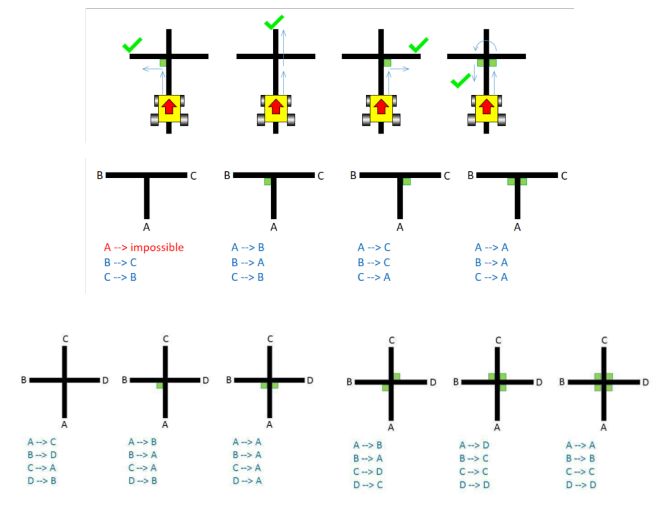
\includegraphics[width=0.9\textwidth]{competencia_rules/reglas.png}
    \caption{\textcolor{orange}{Ejemplo de Intersección}}
    \label{fig:interseccion}
\end{figure}

Para lograrlo, deberán programar el robot utilizando funciones de movimiento y lectura de sensores que hemos aprendido en clases anteriores. Es fundamental que el robot pueda seguir la línea negra con precisión, ya que necesitamos que llegue perpendicularmente a las intersecciones para poder detectarlas correctamente.

A continuación se presentan ejemplos de las líneas que se pueden encontrar en el desafío:

\begin{figure}[H]
    \centering
    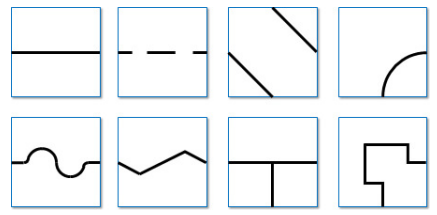
\includegraphics[width=0.9\textwidth]{competencia_rules/tiles.png}
    \caption{\textcolor{orange}{Ejemplo de Líneas en el Circuito}}
    \label{fig:lineas}
\end{figure}

\end{document}
